
%% bare_jrnl_compsoc.tex
%% V1.4b
%% 2015/08/26
%% by Michael Shell
%% See:
%% http://www.michaelshell.org/
%% for current contact information.
%%
%% This is a skeleton file demonstrating the use of IEEEtran.cls
%% (requires IEEEtran.cls version 1.8b or later) with an IEEE
%% Computer Society journal paper.
%%
%% Support sites:
%% http://www.michaelshell.org/tex/ieeetran/
%% http://www.ctan.org/pkg/ieeetran
%% and
%% http://www.ieee.org/

%%*************************************************************************
%% Legal Notice:
%% This code is offered as-is without any warranty either expressed or
%% implied; without even the implied warranty of MERCHANTABILITY or
%% FITNESS FOR A PARTICULAR PURPOSE! 
%% User assumes all risk.
%% In no event shall the IEEE or any contributor to this code be liable for
%% any damages or losses, including, but not limited to, incidental,
%% consequential, or any other damages, resulting from the use or misuse
%% of any information contained here.
%%
%% All comments are the opinions of their respective authors and are not
%% necessarily endorsed by the IEEE.
%%
%% This work is distributed under the LaTeX Project Public License (LPPL)
%% ( http://www.latex-project.org/ ) version 1.3, and may be freely used,
%% distributed and modified. A copy of the LPPL, version 1.3, is included
%% in the base LaTeX documentation of all distributions of LaTeX released
%% 2003/12/01 or later.
%% Retain all contribution notices and credits.
%% ** Modified files should be clearly indicated as such, including  **
%% ** renaming them and changing author support contact information. **
%%*************************************************************************


% *** Authors should verify (and, if needed, correct) their LaTeX system  ***
% *** with the testflow diagnostic prior to trusting their LaTeX platform ***
% *** with production work. The IEEE's font choices and paper sizes can   ***
% *** trigger bugs that do not appear when using other class files.       ***                          ***
% The testflow support page is at:
% http://www.michaelshell.org/tex/testflow/


\documentclass[10pt,journal,compsoc]{IEEEtran}
%
% If IEEEtran.cls has not been installed into the LaTeX system files,
% manually specify the path to it like:
% \documentclass[10pt,journal,compsoc]{../sty/IEEEtran}





% Some very useful LaTeX packages include:
% (uncomment the ones you want to load)


% *** MISC UTILITY PACKAGES ***
%
%\usepackage{ifpdf}
% Heiko Oberdiek's ifpdf.sty is very useful if you need conditional
% compilation based on whether the output is pdf or dvi.
% usage:
% \ifpdf
%   % pdf code
% \else
%   % dvi code
% \fi
% The latest version of ifpdf.sty can be obtained from:
% http://www.ctan.org/pkg/ifpdf
% Also, note that IEEEtran.cls V1.7 and later provides a builtin
% \ifCLASSINFOpdf conditional that works the same way.
% When switching from latex to pdflatex and vice-versa, the compiler may
% have to be run twice to clear warning/error messages.






% *** CITATION PACKAGES ***
%
\ifCLASSOPTIONcompsoc
  % IEEE Computer Society needs nocompress option
  % requires cite.sty v4.0 or later (November 2003)
  \usepackage[nocompress]{cite}
\else
  % normal IEEE
  \usepackage{cite}
\fi
% cite.sty was written by Donald Arseneau
% V1.6 and later of IEEEtran pre-defines the format of the cite.sty package
% \cite{} output to follow that of the IEEE. Loading the cite package will
% result in citation numbers being automatically sorted and properly
% "compressed/ranged". e.g., [1], [9], [2], [7], [5], [6] without using
% cite.sty will become [1], [2], [5]--[7], [9] using cite.sty. cite.sty's
% \cite will automatically add leading space, if needed. Use cite.sty's
% noadjust option (cite.sty V3.8 and later) if you want to turn this off
% such as if a citation ever needs to be enclosed in parenthesis.
% cite.sty is already installed on most LaTeX systems. Be sure and use
% version 5.0 (2009-03-20) and later if using hyperref.sty.
% The latest version can be obtained at:
% http://www.ctan.org/pkg/cite
% The documentation is contained in the cite.sty file itself.
%
% Note that some packages require special options to format as the Computer
% Society requires. In particular, Computer Society  papers do not use
% compressed citation ranges as is done in typical IEEE papers
% (e.g., [1]-[4]). Instead, they list every citation separately in order
% (e.g., [1], [2], [3], [4]). To get the latter we need to load the cite
% package with the nocompress option which is supported by cite.sty v4.0
% and later. Note also the use of a CLASSOPTION conditional provided by
% IEEEtran.cls V1.7 and later.





% *** GRAPHICS RELATED PACKAGES ***
%
\ifCLASSINFOpdf
  \usepackage[pdftex]{graphicx}
  % declare the path(s) where your graphic files are
  % \graphicspath{{../pdf/}{../jpeg/}}
  % and their extensions so you won't have to specify these with
  % every instance of \includegraphics
  % \DeclareGraphicsExtensions{.pdf,.jpeg,.png}
\else
  % or other class option (dvipsone, dvipdf, if not using dvips). graphicx
  % will default to the driver specified in the system graphics.cfg if no
  % driver is specified.
  % \usepackage[dvips]{graphicx}
  % declare the path(s) where your graphic files are
  % \graphicspath{{../eps/}}
  % and their extensions so you won't have to specify these with
  % every instance of \includegraphics
  % \DeclareGraphicsExtensions{.eps}
\fi
% graphicx was written by David Carlisle and Sebastian Rahtz. It is
% required if you want graphics, photos, etc. graphicx.sty is already
% installed on most LaTeX systems. The latest version and documentation
% can be obtained at: 
% http://www.ctan.org/pkg/graphicx
% Another good source of documentation is "Using Imported Graphics in
% LaTeX2e" by Keith Reckdahl which can be found at:
% http://www.ctan.org/pkg/epslatex
%
% latex, and pdflatex in dvi mode, support graphics in encapsulated
% postscript (.eps) format. pdflatex in pdf mode supports graphics
% in .pdf, .jpeg, .png and .mps (metapost) formats. Users should ensure
% that all non-photo figures use a vector format (.eps, .pdf, .mps) and
% not a bitmapped formats (.jpeg, .png). The IEEE frowns on bitmapped formats
% which can result in "jaggedy"/blurry rendering of lines and letters as
% well as large increases in file sizes.
%
% You can find documentation about the pdfTeX application at:
% http://www.tug.org/applications/pdftex






% *** MATH PACKAGES ***
%
%\usepackage{amsmath}
\usepackage{amssymb}
% A popular package from the American Mathematical Society that provides
% many useful and powerful commands for dealing with mathematics.
%
% Note that the amsmath package sets \interdisplaylinepenalty to 10000
% thus preventing page breaks from occurring within multiline equations. Use:
%\interdisplaylinepenalty=2500
% after loading amsmath to restore such page breaks as IEEEtran.cls normally
% does. amsmath.sty is already installed on most LaTeX systems. The latest
% version and documentation can be obtained at:
% http://www.ctan.org/pkg/amsmath





% *** SPECIALIZED LIST PACKAGES ***
%
%\usepackage{algorithmic}
% algorithmic.sty was written by Peter Williams and Rogerio Brito.
% This package provides an algorithmic environment fo describing algorithms.
% You can use the algorithmic environment in-text or within a figure
% environment to provide for a floating algorithm. Do NOT use the algorithm
% floating environment provided by algorithm.sty (by the same authors) or
% algorithm2e.sty (by Christophe Fiorio) as the IEEE does not use dedicated
% algorithm float types and packages that provide these will not provide
% correct IEEE style captions. The latest version and documentation of
% algorithmic.sty can be obtained at:
% http://www.ctan.org/pkg/algorithms
% Also of interest may be the (relatively newer and more customizable)
% algorithmicx.sty package by Szasz Janos:
% http://www.ctan.org/pkg/algorithmicx




% *** ALIGNMENT PACKAGES ***
%
%\usepackage{array}
% Frank Mittelbach's and David Carlisle's array.sty patches and improves
% the standard LaTeX2e array and tabular environments to provide better
% appearance and additional user controls. As the default LaTeX2e table
% generation code is lacking to the point of almost being broken with
% respect to the quality of the end results, all users are strongly
% advised to use an enhanced (at the very least that provided by array.sty)
% set of table tools. array.sty is already installed on most systems. The
% latest version and documentation can be obtained at:
% http://www.ctan.org/pkg/array


% IEEEtran contains the IEEEeqnarray family of commands that can be used to
% generate multiline equations as well as matrices, tables, etc., of high
% quality.




% *** SUBFIGURE PACKAGES ***
%\ifCLASSOPTIONcompsoc
%  \usepackage[caption=false,font=footnotesize,labelfont=sf,textfont=sf]{subfig}
%\else
%  \usepackage[caption=false,font=footnotesize]{subfig}
%\fi
% subfig.sty, written by Steven Douglas Cochran, is the modern replacement
% for subfigure.sty, the latter of which is no longer maintained and is
% incompatible with some LaTeX packages including fixltx2e. However,
% subfig.sty requires and automatically loads Axel Sommerfeldt's caption.sty
% which will override IEEEtran.cls' handling of captions and this will result
% in non-IEEE style figure/table captions. To prevent this problem, be sure
% and invoke subfig.sty's "caption=false" package option (available since
% subfig.sty version 1.3, 2005/06/28) as this is will preserve IEEEtran.cls
% handling of captions.
% Note that the Computer Society format requires a sans serif font rather
% than the serif font used in traditional IEEE formatting and thus the need
% to invoke different subfig.sty package options depending on whether
% compsoc mode has been enabled.
%
% The latest version and documentation of subfig.sty can be obtained at:
% http://www.ctan.org/pkg/subfig




% *** FLOAT PACKAGES ***
%
%\usepackage{fixltx2e}
% fixltx2e, the successor to the earlier fix2col.sty, was written by
% Frank Mittelbach and David Carlisle. This package corrects a few problems
% in the LaTeX2e kernel, the most notable of which is that in current
% LaTeX2e releases, the ordering of single and double column floats is not
% guaranteed to be preserved. Thus, an unpatched LaTeX2e can allow a
% single column figure to be placed prior to an earlier double column
% figure.
% Be aware that LaTeX2e kernels dated 2015 and later have fixltx2e.sty's
% corrections already built into the system in which case a warning will
% be issued if an attempt is made to load fixltx2e.sty as it is no longer
% needed.
% The latest version and documentation can be found at:
% http://www.ctan.org/pkg/fixltx2e


%\usepackage{stfloats}
% stfloats.sty was written by Sigitas Tolusis. This package gives LaTeX2e
% the ability to do double column floats at the bottom of the page as well
% as the top. (e.g., "\begin{figure*}[!b]" is not normally possible in
% LaTeX2e). It also provides a command:
%\fnbelowfloat
% to enable the placement of footnotes below bottom floats (the standard
% LaTeX2e kernel puts them above bottom floats). This is an invasive package
% which rewrites many portions of the LaTeX2e float routines. It may not work
% with other packages that modify the LaTeX2e float routines. The latest
% version and documentation can be obtained at:
% http://www.ctan.org/pkg/stfloats
% Do not use the stfloats baselinefloat ability as the IEEE does not allow
% \baselineskip to stretch. Authors submitting work to the IEEE should note
% that the IEEE rarely uses double column equations and that authors should try
% to avoid such use. Do not be tempted to use the cuted.sty or midfloat.sty
% packages (also by Sigitas Tolusis) as the IEEE does not format its papers in
% such ways.
% Do not attempt to use stfloats with fixltx2e as they are incompatible.
% Instead, use Morten Hogholm'a dblfloatfix which combines the features
% of both fixltx2e and stfloats:
%
% \usepackage{dblfloatfix}
% The latest version can be found at:
% http://www.ctan.org/pkg/dblfloatfix




%\ifCLASSOPTIONcaptionsoff
%  \usepackage[nomarkers]{endfloat}
% \let\MYoriglatexcaption\caption
% \renewcommand{\caption}[2][\relax]{\MYoriglatexcaption[#2]{#2}}
%\fi
% endfloat.sty was written by James Darrell McCauley, Jeff Goldberg and 
% Axel Sommerfeldt. This package may be useful when used in conjunction with 
% IEEEtran.cls'  captionsoff option. Some IEEE journals/societies require that
% submissions have lists of figures/tables at the end of the paper and that
% figures/tables without any captions are placed on a page by themselves at
% the end of the document. If needed, the draftcls IEEEtran class option or
% \CLASSINPUTbaselinestretch interface can be used to increase the line
% spacing as well. Be sure and use the nomarkers option of endfloat to
% prevent endfloat from "marking" where the figures would have been placed
% in the text. The two hack lines of code above are a slight modification of
% that suggested by in the endfloat docs (section 8.4.1) to ensure that
% the full captions always appear in the list of figures/tables - even if
% the user used the short optional argument of \caption[]{}.
% IEEE papers do not typically make use of \caption[]'s optional argument,
% so this should not be an issue. A similar trick can be used to disable
% captions of packages such as subfig.sty that lack options to turn off
% the subcaptions:
% For subfig.sty:
% \let\MYorigsubfloat\subfloat
% \renewcommand{\subfloat}[2][\relax]{\MYorigsubfloat[]{#2}}
% However, the above trick will not work if both optional arguments of
% the \subfloat command are used. Furthermore, there needs to be a
% description of each subfigure *somewhere* and endfloat does not add
% subfigure captions to its list of figures. Thus, the best approach is to
% avoid the use of subfigure captions (many IEEE journals avoid them anyway)
% and instead reference/explain all the subfigures within the main caption.
% The latest version of endfloat.sty and its documentation can obtained at:
% http://www.ctan.org/pkg/endfloat
%
% The IEEEtran \ifCLASSOPTIONcaptionsoff conditional can also be used
% later in the document, say, to conditionally put the References on a 
% page by themselves.




% *** PDF, URL AND HYPERLINK PACKAGES ***
%
%\usepackage{url}
% url.sty was written by Donald Arseneau. It provides better support for
% handling and breaking URLs. url.sty is already installed on most LaTeX
% systems. The latest version and documentation can be obtained at:
% http://www.ctan.org/pkg/url
% Basically, \url{my_url_here}.





% *** Do not adjust lengths that control margins, column widths, etc. ***
% *** Do not use packages that alter fonts (such as pslatex).         ***
% There should be no need to do such things with IEEEtran.cls V1.6 and later.
% (Unless specifically asked to do so by the journal or conference you plan
% to submit to, of course. )


% correct bad hyphenation here
%\hyphenation{op-tical net-works semi-conduc-tor}

\newcommand{\tup}[1]{{\langle #1 \rangle}}
\newcommand{\pre}{\mathsf{pre}}    % precondition
\newcommand{\eff}{\mathsf{eff}}    % effect
\newcommand{\cond}{\mathsf{cond}}  % condition
\newcommand{\dur}{\mathsf{dur}}    % duration
\newcommand{\obs}{\mathsf{obs}}    % observation
\newcommand{\start}{\mathsf{start}}% start
\newcommand{\en}{\mathsf{end}}     % end
\newcommand{\til}{\mathsf{til}}    % TIL
\newcommand{\supp}{\mathsf{sup}}   % sup
\newcommand{\tim}{\mathsf{time}}   % time
\newcommand{\reqs}{\mathsf{req\_{start}}} % req_start
\newcommand{\reqe}{\mathsf{req\_{end}}}   % req_end
\newcommand{\ini}{\mathsf{init}}   % init
\newcommand{\goal}{\mathsf{goal}}  % goal
%\newcommand{\add}{\mathsf{add}}
%\newcommand{\del}{\mathsf{del}}


\begin{document}
%
% paper title
% Titles are generally capitalized except for words such as a, an, and, as,
% at, but, by, for, in, nor, of, on, or, the, to and up, which are usually
% not capitalized unless they are the first or last word of the title.
% Linebreaks \\ can be used within to get better formatting as desired.
% Do not put math or special symbols in the title.
\title{One-Shot Learning of Temporal Features on Action Models via Constraint Programming}
%
%
% author names and IEEE memberships
% note positions of commas and nonbreaking spaces ( ~ ) LaTeX will not break
% a structure at a ~ so this keeps an author's name from being broken across
% two lines.
% use \thanks{} to gain access to the first footnote area
% a separate \thanks must be used for each paragraph as LaTeX2e's \thanks
% was not built to handle multiple paragraphs
%
%
%\IEEEcompsocitemizethanks is a special \thanks that produces the bulleted
% lists the Computer Society journals use for "first footnote" author
% affiliations. Use \IEEEcompsocthanksitem which works much like \item
% for each affiliation group. When not in compsoc mode,
% \IEEEcompsocitemizethanks becomes like \thanks and
% \IEEEcompsocthanksitem becomes a line break with idention. This
% facilitates dual compilation, although admittedly the differences in the
% desired content of \author between the different types of papers makes a
% one-size-fits-all approach a daunting prospect. For instance, compsoc 
% journal papers have the author affiliations above the "Manuscript
% received ..."  text while in non-compsoc journals this is reversed. Sigh.

\author{Antonio~Garrido and~Sergio~Jim\'enez}

%\IEEEcompsocitemizethanks{\IEEEcompsocthanksitem M. Shell was with the Department
%of Electrical and Computer Engineering, Georgia Institute of Technology, Atlanta,
%GA, 30332.\protect\\
%% note need leading \protect in front of \\ to get a newline within \thanks as
%% \\ is fragile and will error, could use \hfil\break instead.
%E-mail: @dsic.upv.es
%\IEEEcompsocthanksitem Universitat Politecnica de Valencia, Camino de Vera s/n, 46022, Valencia (Spain).}% <-this % stops an unwanted space
%\thanks{thanks}
\author{Antonio~Garrido
	and~Sergio~Jim\'enez% <-this % stops a space
	\IEEEcompsocitemizethanks{\IEEEcompsocthanksitem A. Garrido and S. Jim\'enez are with VRAIN, Valencian Research Institute for Artificial Intelligence. Universitat Politecnica de Valencia, Camino de Vera s/n, 46022. Valencia (Spain).\protect\\
		% note need leading \protect in front of \\ to get a newline within \thanks as
		% \\ is fragile and will error, could use \hfil\break instead.
		E-mail: \{agarridot,serjice\}@dsic.upv.es
		%\IEEEcompsocthanksitem
	}% <-this % stops an unwanted space
	\thanks{}}




% note the % following the last \IEEEmembership and also \thanks - 
% these prevent an unwanted space from occurring between the last author name
% and the end of the author line. i.e., if you had this:
% 
% \author{....lastname \thanks{...} \thanks{...} }
%                     ^------------^------------^----Do not want these spaces!
%
% a space would be appended to the last name and could cause every name on that
% line to be shifted left slightly. This is one of those "LaTeX things". For
% instance, "\textbf{A} \textbf{B}" will typeset as "A B" not "AB". To get
% "AB" then you have to do: "\textbf{A}\textbf{B}"
% \thanks is no different in this regard, so shield the last } of each \thanks
% that ends a line with a % and do not let a space in before the next \thanks.
% Spaces after \IEEEmembership other than the last one are OK (and needed) as
% you are supposed to have spaces between the names. For what it is worth,
% this is a minor point as most people would not even notice if the said evil
% space somehow managed to creep in.



% The paper headers
%\markboth{Journal of \LaTeX\ Class Files,~Vol.~14, No.~8, August~2015}%
%{Shell \MakeLowercase{\textit{et al.}}: Bare Demo of IEEEtran.cls for Computer Society Journals}
% The only time the second header will appear is for the odd numbered pages
% after the title page when using the twoside option.
% 
% *** Note that you probably will NOT want to include the author's ***
% *** name in the headers of peer review papers.                   ***
% You can use \ifCLASSOPTIONpeerreview for conditional compilation here if
% you desire.



% The publisher's ID mark at the bottom of the page is less important with
% Computer Society journal papers as those publications place the marks
% outside of the main text columns and, therefore, unlike regular IEEE
% journals, the available text space is not reduced by their presence.
% If you want to put a publisher's ID mark on the page you can do it like
% this:
%\IEEEpubid{0000--0000/00\$00.00~\copyright~2015 IEEE}
% or like this to get the Computer Society new two part style.
%\IEEEpubid{\makebox[\columnwidth]{\hfill 0000--0000/00/\$00.00~\copyright~2015 IEEE}%
%\hspace{\columnsep}\makebox[\columnwidth]{Published by the IEEE Computer Society\hfill}}
% Remember, if you use this you must call \IEEEpubidadjcol in the second
% column for its text to clear the IEEEpubid mark (Computer Society jorunal
% papers don't need this extra clearance.)



% use for special paper notices
%\IEEEspecialpapernotice{(Invited Paper)}



% for Computer Society papers, we must declare the abstract and index terms
% PRIOR to the title within the \IEEEtitleabstractindextext IEEEtran
% command as these need to go into the title area created by \maketitle.
% As a general rule, do not put math, special symbols or citations
% in the abstract or keywords.
\IEEEtitleabstractindextext{%
	\begin{abstract}
	This work proposes a novel constraint programming approach for learning the temporal features of durative actions in an expressive temporal planning model with overlapping actions, which makes it suitable for learning in multi-agent environments.
	We analyze the extreme scenario, where just a single (one-shot) partial observation of the execution of a temporal plan is available, to learn the distribution of conditions/effects and estimate the durations, resulting in a consistent constraint model.
	Our approach automatically builds a purely declarative formulation that models time-stamps for actions, causal link relationships (conditions and effects), threats and effect interferences that appear in planning. It also accommodates a different range of expressiveness, subsuming the PDDL2.1 temporal semantics. Our formulation is simple but effective, and is not only valid for learning, but also for plan validation, as shown in its evaluation that returns high precision and success ratios. Finally, our formulation is solver-independent, meaning that an arbitrary CSP solver can be used for its resolution.
	\end{abstract}

% Note that keywords are not normally used for peerreview papers.
%\begin{IEEEkeywords}
%One-shot learning action models, Temporal planning, Partial observability, Constraint programming.
%\end{IEEEkeywords}
}


% make the title area
\maketitle


% To allow for easy dual compilation without having to reenter the
% abstract/keywords data, the \IEEEtitleabstractindextext text will
% not be used in maketitle, but will appear (i.e., to be "transported")
% here as \IEEEdisplaynontitleabstractindextext when the compsoc 
% or transmag modes are not selected <OR> if conference mode is selected 
% - because all conference papers position the abstract like regular
% papers do.
\IEEEdisplaynontitleabstractindextext
% \IEEEdisplaynontitleabstractindextext has no effect when using
% compsoc or transmag under a non-conference mode.



% For peer review papers, you can put extra information on the cover
% page as needed:
% \ifCLASSOPTIONpeerreview
% \begin{center} \bfseries EDICS Category: 3-BBND \end{center}
% \fi
%
% For peerreview papers, this IEEEtran command inserts a page break and
% creates the second title. It will be ignored for other modes.
\IEEEpeerreviewmaketitle



\IEEEraisesectionheading{\section{Introduction}\label{sec:introduction}}
% Computer Society journal (but not conference!) papers do something unusual
% with the very first section heading (almost always called "Introduction").
% They place it ABOVE the main text! IEEEtran.cls does not automatically do
% this for you, but you can achieve this effect with the provided
% \IEEEraisesectionheading{} command. Note the need to keep any \label that
% is to refer to the section immediately after \section in the above as
% \IEEEraisesectionheading puts \section within a raised box.




% The very first letter is a 2 line initial drop letter followed
% by the rest of the first word in caps (small caps for compsoc).
% 
% form to use if the first word consists of a single letter:
% \IEEEPARstart{A}{demo} file is ....
% 
% form to use if you need the single drop letter followed by
% normal text (unknown if ever used by the IEEE):
% \IEEEPARstart{A}{}demo file is ....
% 
% Some journals put the first two words in caps:
% \IEEEPARstart{T}{his demo} file is ....
% 

\IEEEPARstart{A}{utomated} planning is the model-based approach for the task of selecting the actions that achieve a given set of goals starting from a given initial state. {\em Classical planning} (\textit{aka} STRIPS planning) is the vanilla model for planning and it assumes: fully observable states under a deterministic world, instantaneous actions, and goals that are exclusively referred to the last state reached by a plan~\cite{geffner2013concise,ghallab2004automated}. Beyond classical planning, there is a bunch of more expressive planning models that relax the previous assumptions to compute more detailed solutions than classical plans~\cite{ghallab2004automated}.


{\em Temporal planning} is one of these more expressive planning models, as it relaxes the assumption of instantaneous actions~\cite{fox2003pddl2}. Temporal actions have durations and conditions/effects that must hold/happen at different times, which means that temporal actions can be executed in parallel and overlap in several ways~\cite{cushing2007temporal}. Consequently, valid solution plans for temporal planning problems need to indicate the precise time-stamp when an action starts and ends~\cite{howey2004val}.

\subsection{Motivation}

Despite the potential of state-of-the-art planners, its applicability to the real world is still somewhat limited because of the difficulty and time-consuming of manually specifying correct and complete planning models~\cite{kambhampati2007model,ZhuoYHL10}, particularly in expressive temporal action languages~\cite{cushing2007temporal}. The more expressive the planning model is, the more evident becomes this knowledge engineering bottleneck, which jeopardizes the usability of AI planning technology. This has led to a growing interest in the planning community for the learning of action models, as a cognitive task~\cite{Baker2009}, to improve their quality and reduce the human effort~\cite{jimenez2012review,ZhuoYHL10}. 
The objective of this learning task is to understand and predict action models
%by computing the actions' conditions and effects 
that are {\em consistent} with a set of noiseless observations (defined as some sequence of state changes, input constraints, world transitions, expert demonstrations or plan traces/logs). Model learning from observation of past behavior provides indirect, but very valuable, information to hypothesize the action models, thus helping future planning decisions and recommendations of preference models~\cite{Aggarwal2016}. This is specially interesting for proactive assistants when recognizing activities of multiple (human or software) agents to assist them in their daily activities and, as the ultimate frontier, to generate personalized recommendations, predict and anticipate their needs or actions.


Most approaches for learning planning action models are purely inductive and often require large datasets of observations, e.g. thousands of plan observations, to compute a statistically significant model that minimizes some error metric over the observations~\cite{kuvcera2018louga,MouraoZPS12,yang2007learning,ZhuoYHL10,zhuo2013action}. Defining model learning as an optimization task over a large set of observations does not guarantee completeness (the learned model may fail to explain an observation), nor correctness (the states induced by the execution of the plan generated with the model may contain contradictory information). 
Further, in many real-world applications it is expensive to collect large datasets of observations for training~\cite{Jialin2010}, or even impossible.
This often happens when the number of samples is limited or when a human needs to perform repetitive actions (learning by demonstration).
Therefore, reducing the effort to deal with tractable datasets is desirable~\cite{Jialin2010}.


Learning an action model for classical planning involves computing the actions' conditions and effects that are consistent with the input observations.
Learning classical action models has been addressed by different approaches~\cite{arora2018review}. Since pioneering learning systems like ARMS~\cite{yang2007learning}, we have seen systems able to learn STRIPS action models with quantifiers~\cite{AmirC08,ZhuoYHL10}, from noisy actions or states~\cite{MouraoZPS12,zhuo2013action}, from null state information~\cite{cresswell2013acquiring}, from incomplete domain models~\cite{ZhuoK17,ZhuoNK13}, or from partially observed plan traces~\cite{Zhuo2014}. But, to our knowledge, none of these systems deals with durative actions to learn their temporal features. 
Learning the temporal features means: i) to identify how actions' conditions and effects are temporally distributed in the action execution; ii) to estimate the action duration according to the observations; and, after all, iii) to model a class of highly expressive durative actions that meet the challenges of real-world planning.
Roughly speaking, learning a classical action model aims to decide which are the conditions/effects, whereas learning the temporal features aims to decide when and how they are used. And these two learning tasks are asymptotically very complex.


As a motivating example, let us assume a logistics scenario. When driving a truck between two locations, the road should be available all over the execution of the action. However, if we use a plane for transportation, we will only need an airport at the beginning+end of the action.
On the other hand, given a full logistics trace, we can deduce the precise duration of an action. But if observations are partial, we might only observe when the trip starts, but not the exact time when it ends (traffic congestion may affect). Or, analogously, we might know when the trip ends but be unsure about when it started. 
In classical planning none of the previous statements entails difficulty: the distribution of conditions/effects is fixed, as they are always allocated at the start/end of the action, respectively, and all actions have unitary duration, which is not very realistic.
In temporal planning, if a human modeler perfectly knows the semantics of the logistics actions, learning the temporal features may not be a complicated task either. But, without that expert knowledge, if the human has to distribute conditions arbitrarily named $\{p, q, r\}$, effects $\{not-p, not-q, s\}$ and estimate valid durations for unknown actions $\{a1, a2, a3\}$ over a set of partial observations, the task becomes much more complex. The learning task induces many assignments that need to fit a complex puzzle, because not all combinations are valid and they depend on the interactions with other actions, observations and constraints. And surely this is not easy for a human. 
Eventually, learning the temporal features will allow us: i) to better understand the insights of the logistics in terms of what is possible (or not) and why, because the model is consistent with the observed data; ii) to suggest changes that can improve the model originally created by a human, e.g. re-distributing the actions' conditions, provided they still explain the observations; and iii) to automatically elaborate similar models for similar scenarios (i.e. knowledge transfer or transfer learning~\cite{Jialin2010}), such as public transit for commuters, tourists or people in general in metropolitan areas ---\textit{aka} smart urban mobility.


\subsection{Proposed Work}

Based on a classical model of actions, this paper analyzes a novel application of Constraint Programming (CP) for the {\em one-shot learning} of the temporal features; that is, the extreme case of learning from a single and partially specified model observed from the execution of a temporal plan. On the one hand, our main contribution in the field of knowledge engineering is a constraint formulation for a very expressive temporal planning model that follows the work in~\cite{garrido2009constraint}. Such a work proposes a CP formulation, automatically generated from a given model of actions, to be used for planning and/or scheduling a whole plan.
We keep the philosophy of using CP but, contrary to~\cite{garrido2009constraint}, we address the inverse task now: learn the temporal features of an action model given a plan trace and a partial model of actions. Intuitively, the input model of actions used in~\cite{garrido2009constraint} is our output now, as we are interested in learning/playing the designer's role, \emph{w.r.t} the temporal features, rather than in planning. 
On the other hand, another contribution is to learn as much knowledge as possible from the lowest amount of observations.
Rather than using a machine learning approach that builds a statistical model that requires huge datasets, we exploit CP inference for deductive reasoning on arbitrary size plan traces.


In our work we focus on the temporal aspects and rely on the classical conditions+effects. Although this could seem a limitation of our proposal, there is no need to deliberately learn them again as they can be obtained by existing approaches, previously modeled by a human, or observed. But (partial) observations may now refer to the execution of overlapping durative actions, in opposition to most of the existing approaches that work with sequential non-durative actions. Working with overlapping makes our approach suitable for learning in multi-agent environments, which is also a contribution to deal with realistic scenarios. Finally, the paper evidences that the learning of temporal features strongly resembles the task of synthesizing and validating a plan that satisfies all the imposed constraints or, in other words, that is consistent with the noiseless input observations. This is our last contribution: a unified CP formulation for both learning and plan validation, which supports temporal models and addresses plan validation of partial action models beyond the functionality of standard validators~\cite{howey2004val}.


The paper is organized as follows. Section~\ref{sec:background} introduces the background and terminology used. Section~\ref{sec:learningTemporalFeatures} formalizes the learning task of temporal features, and exemplifies the difficulty of such learning and the huge number of combinations that appear. In Section~\ref{sec:CPformulation} we elaborate our CP formulation for learning, presenting the variables,  constraints and some simple heuristics. It also shows how our formulation is flexible enough to be used for plan validation.
The evaluation and experimental results are shown in Section~\ref{sec:evaluation}. Finally, Section~\ref{sec:conclusions} concludes the paper and proposes some future work.


\section{Background and Terminology}
\label{sec:background}

This section formalizes the {\em classical} and {\em temporal} planning models that we follow in this work, as well as the {\em Constraint Satisfaction Problem}.


\subsection{Classical Planning}
\label{sec:classicalplanning}


Let $F$ be a set of facts that represent propositional variables.
Without loss of generality, we assume that $F$ does not contain conflicting values $f$ and $not-f$.
A state $s$ is a full assignment of boolean values to variables, $|s|=|F|$, so the size of the state space is $2^{|F|}$.
A {\em classical planning problem} is a tuple $\tup{F,I,G,A}$, where $I$ is the initial state, $G \subseteq F$ is a set of goal conditions over $F$, and $A$ is the set of actions that modify states. We assume that actions are grounded from action schemas or operators, as in PDDL (Planning Domain Definition Language~\cite{fox2003pddl2,ghallab2004automated}). A grounded action is a schema where all the parameters are fully instantiated.

Each action $a \in A$ has a set of preconditions $\pre(a)$ and a set of effects $\eff(a)=\{\eff^+(a) \cup \eff^-(a)\}$; $\pre(a), \eff^+(a), \eff^-(a) \subseteq F$. $\pre(a)$ must hold before $a$ starts (this is why they are named \emph{pre}conditions), whereas $\eff(a)$ happen when $a$ ends. This way, $a$ is applicable in a state $s$ if $\pre(a) \subseteq s$. When $a$ is executed, a new state, the successor of $s$, is created that results of applying $\eff(a)$ on $s$. Typically, $\eff(a)$ is formed by positive and negative/delete effects ($\eff^+(a)$ and $\eff^-(a)$, which are asserted and retracted, respectively). Fig.~\ref{fig:exampleactions1} shows an example of two classical actions for a logistics scenario, from the \emph{driverlog} domain of the International Planning Competition (IPC).\footnote{{\scriptsize \texttt{www.icaps-conference.org/index.php/Main/Competitions}}} Action \texttt{board-truck} boards a driver on an empty truck at a given location. In \texttt{drive-truck} a truck is driven between two locations, provided there is a link between them.

\begin{figure}
	{\scriptsize
	\begin{tabular}{p{\textwidth}}
		\begin{verbatim}
		(:action board-truck
		 :parameters (?d - driver ?t - truck ?l - location)
		 :precondition (and (at ?d ?l) (empty ?t) (at ?t ?l))
		 :effect (and (not (at ?d ?l)) (not (empty ?t)) 
		              (driving ?d ?t)))
		
		(:action drive-truck
		 :parameters (?t - truck ?from - location ?to - location 
		              ?d - driver)
		 :precondition (and (at ?t ?from) (link ?from ?to) 
		                    (driving ?d ?t))
		 :effect (and (not (at ?t ?from)) (at ?t ?to)))
		\end{verbatim}
	\end{tabular}
	}
	\caption{\small PDDL schema for two classical actions from the {\em driverlog} domain.}
	\label{fig:exampleactions1}
\end{figure}


In this work we define a plan for a classical planning problem as a set of pairs $\tup{(a_1,t_1),(a_2,t_2)\ldots (a_n,t_n)}$. Each $(a_i,t_i)$ pair contains an instantaneous action $a_i$ and the planning step $t_i$ when $a_i$ starts.
This action sequence induces a state sequence $\tup{s_1,s_2\ldots s_n}$, where each $a_i$ is applicable in $s_{i-1}$, being $s_0=I$, and generates state $s_i$. In every valid plan $G\subseteq s_n$, i.e. the goal condition is satisfied in the last state.
In general terms, classical plans can be sequential plans, where only one action is executed at each planning step, or parallel plans, where several actions can be executed at the same planning step.




\subsection{Temporal Planning}
\label{sec:temporalplanning}

A {\em temporal planning problem} is also a tuple $\tup{F,I,G,A}$ where $F$, $I$ and $G$ are defined like in classical planning, and $A$ represents the set of {\em durative actions}. There are several options that allow for a high expressiveness of durative actions. On the one hand, an action can have a fixed duration, a duration that ranges within an interval or a distribution of durations. On the other hand, actions may have conditions/effects annotated at different times, such as conditions that must hold some time before the action starts, effects that happen just when the action starts, in the middle of the action or some time after the action finishes~\cite{garrido2009constraint}.

A popular model for temporal planning is given by PDDL2.1~\cite{fox2003pddl2}, a language that somewhat restricts temporal expressiveness, which defines a durative action $a$ with the following elements:

\begin{itemize}
	
	\item $\dur(a)$, a positive value for the action duration.
	
	\item $\cond_s(a), \cond_o(a), \cond_e(a)$. Unlike the \emph{pre}conditions of a classical action, now conditions must hold before $a$ ({\em at start}), during the entire execution of $a$ ({\em over all}) or when $a$ finishes ({\em at end}), respectively. In the simplest case, $\cond_s(a) \cup \cond_o(a) \cup \cond_e(a) = \pre(a).$\footnote{In classical planning, $\pre(a)=\{p,not-p\}$ is contradictory. In temporal planning, $\cond_s(a)=\{p\}$ and $\cond_e(a)=\{not-p\}$ is a possible situation, though very unusual.}
	%Note that $\cond_s(a) \cup \cond_o(a) \cup \cond_e(a) \subseteq \pre(a)$, since $\cond_s(a)=\{p\}$ and $\cond_e(a)=\{not-p\}$ is, for instance, now possible.	
	
	\item $\eff_s(a)$ and $\eff_e(a)$. Now effects can happen {\em at start} or {\em at end} of $a$, respectively, and can still be positive or negative. Again, in the simplest case $\eff_s(a) \cup \eff_e(a) = \eff(a)$.\footnote{In classical planning, $\eff(a)=\{p,not-p\}$ is contradictory. In temporal planning, $\eff_s(a)=\{not-p\}$ and $\eff_e(a)=\{p\}$ is a possible and frequent situation to block/unblock a resource $p$ used within $a$.}
	%Again, $\eff_s(a) \cup \eff_e(a) \subseteq \eff(a)$.
	
\end{itemize}


%Despite durative actions are no longer instantaneous in PDDL2.1, {\em at start} and {\em at end} conditions are checked instantaneously.

The semantics of a PDDL2.1 durative action $a$ can be defined in terms of two discrete events, $\start(a)$ and $\en(a)=\start(a)+\dur(a)$. This means that if action $a$ starts on state $s$, $\cond_s(a)$ must hold in $s$; and ending $a$ in state $s'$ means $\cond_e(a)$ holds in $s'$. {\em Over all} conditions must hold at any state between $s$ and $s'$ or, in other words, throughout interval $[\start(a)..\en(a)]$.
Analogously, {\em at start} and {\em at end} effects are instantaneously applied at states $s$ and $s'$, respectively ---continuous effects are not considered.
Fig.~\ref{fig:exampleactions2} shows two durative actions that extend the classical actions of Fig.~\ref{fig:exampleactions1}. Now \texttt{board-truck} has a fixed duration whereas in \texttt{drive-truck} the duration depends on the two locations.

\begin{figure}
	{\scriptsize
	\begin{tabular}{p{\textwidth}}
		\begin{verbatim}
		(:durative-action board-truck
		 :parameters (?d - driver ?t - truck ?l - location)
		 :duration (= ?duration 2)
		 :condition (and (at start (at ?d ?l)) 
		                 (at start (empty ?t))
		                 (over all (at ?t ?l)))
		 :effect (and (at start (not (at ?d ?l))) 
		              (at start (not (empty ?t)))
		              (at end (driving ?d ?t))))
		
		(:durative-action drive-truck
		 :parameters (?t - truck ?from - location ?to - location 
		              ?d - driver)
		 :duration (= ?duration (driving-time ?from ?to))
		 :condition (and (at start (at ?t ?from)) 
		                 (at start (link ?from ?to))
		                 (over all (driving ?d ?t)))
		 :effect (and (at start (not (at ?t ?from))) 
		              (at end (at ?t ?to))))
		\end{verbatim}
	\end{tabular}
	}
	\caption{\small PDDL2.1 schema for two durative actions from the {\em driverlog} domain.}
	\label{fig:exampleactions2}
\end{figure}



PDDL2.2 is an evolution of PDDL2.1 that extends the initial state $I$ with the notion of {\em Timed Initial Literals}~\cite{hoffmann2005} ($\til(f,t)$ or $\til(not-f,t)$). A TIL is introduced as a way of asserting or retracting a fact $f \in F$ at a certain time $t$, independently of the actions in the plan.\footnote{Intuitively, the information in $I$ can be seen as a particular case of TILs with time $t=0$.} TILs are very useful in temporal planning to define exogenous happenings; for instance, a time window when a warehouse is open in a logistics scenario ($\til(open,8)$ and $\til(not-open,20)$).


A temporal plan is a set of pairs $\tup{(a_1,t_1),(a_2,t_2)\ldots (a_n,t_n)}$. Each $(a_i,t_i)$ pair contains a durative action $a_i$ and $t_i=\start(a_i)$.
This temporal plan induces a state sequence formed by the union of all states $\{s_{t_i}, s_{t_i+\dur(a_i)}\}$, where there exists a state $s_{0}=I$, and $G\subseteq s_{end}$, being $s_{end}$ the last state induced by the plan.
Though a sequential temporal plan is syntactically possible, it is semantically useless. Consequently, temporal plans are always given as parallel plans, which is essential for multi-agent planning.


\subsection{Constraint Satisfaction Problems}
\label{sec:csp}

A {\em Constraint Satisfaction Problem} (CSP) is defined as the tuple $\tup{V,D,C}$, where:

\begin{itemize}
	
	\item $V=\tup{v_1,v_2 \ldots v_n}$ is a set of $n$ finite domain variables.
	
	\item $D=\tup{D_{v_1},D_{v_2} \ldots D_{v_n}}$ are the respective domains defining the set of possible values for each variable $v_i \in V$.
	
	\item $C=\tup{c_1,c_2 \ldots c_m}$ is a set of constraints binding the possible values of the variables in $V$. Every constraint $c_i\in C$ is defined as a pair $c_i=\tup{V_i,R_i}$, where:
	\begin{itemize}
		\item $V_i\subseteq V$ is a subset of $k\leq n$ variables.
		\item $R_i$ is a $k$-ary relation on the corresponding subset of domains.
	\end{itemize}
\end{itemize}

An evaluation $ev_i$ satisfies a constraint $c_i=\tup{V_i,R_i}$ if the values of $ev_i$ assigned to the variables in $V_i$ satisfy the relation $R_i$. An evaluation of values to all variables in $V$ is {\em consistent} if it does not violate any of the constraints in $C$, i.e. it is a solution for the CSP $\tup{V,D,C}$. Note that we deal with a satisfaction problem and, consequently, the CSP can have many solutions.



\section{One-Shot Learning of Temporal Features}
\label{sec:learningTemporalFeatures}


\subsection{Learning Task}
\label{sec:learningtask}

We define our one-shot learning task of temporal features in an action model as a tuple $\tup{F,I,G,A?,O}$, where:

\begin{itemize}
	
	\item $\tup{F,I,G,A?}$ is a temporal planning problem in which actions are partially specified. Actions in $A?$ are those observed in the plan trace. They are partially specified because we do not know the exact structure in terms of distribution of conditions/effects nor the duration. In this work we assume that, for each action $a \in A?$, we only know $\pre(a)$ and $\eff(a)$, as this information can be extracted from the classical version of the planning problem, from prior knowledge we have on the problem, or given by an expert.
	
	\item $O$ is the sequence of observations, provided by a sensor or human observer, corresponding to a plan trace which contains the time when an action $a$ in $A?$ starts ($\start(a)$) or ends ($\en(a)$). In a partial observation context, we might observe the start of the action and/or its end. If we observe both $\start(a)$ and $\en(a)$ we can easily calculate $\dur(a)$; otherwise $\dur(a)$ needs to be estimated. In our work, we assume only one in $\{\start(a), \en(a)\}$ is observed to minimize the number of required (partial) observations. In practice, sensors usually observe changing properties of the word and deduce whether a proposition is true or false at a given time. In order to simulate the observation of the execution of action $a$, we can use dummy propositions $\mathsf{is\_start}(a), \mathsf{is\_end}(a)$ with values true/false, representing whether the action starts or ends.% at a given time.	
			
\end{itemize}


Note that our definition of learning task requires the minimal amount of input knowledge on the states: only the result of the plan execution is observed. 
More particularly, we do not observe any intermediate state in pursuit of minimizing the number of observations. We only require $I$, as a full state, and $G$, as a partial state of goals.\footnote{Other learning tasks can also include intermediate states and input knowledge on static information, which makes the learning task easier to be solved~\cite{aineto2018icaps}.} A solution to this learning task is a fully specified model of temporal actions $\mathcal{A}$, with all actions of $A?$, where the duration and distribution of conditions/effects is completely specified. In other words, for each action $a \in A?$, we have its equivalent version in $\mathcal{A}$ where we have learned $\dur(a)$, $\cond_s(a)$, $\cond_o(a)$, $\cond_e(a)$, $\eff_s(a)$ and $\eff_e(a)$.
Actions in $\mathcal{A}$ must be consistent with the partial specification given in $A?$, which means having exactly the same conditions and effects, starting and/or ending as observed in $O$, and inducing a temporal plan from $I$ that satisfies $G$. Intuitively, $\mathcal{A}$ is a solution to the learning task if it explains all the observations (completeness) and its subjacent temporal model implies no contradictions in the states induced by their execution (correctness).

As can be noticed, the learned model $\mathcal{A}$ must satisfy all the constraints imposed by both the partially specified model $A?$ and the observations $O$.
%Loosely speaking, the partially specified model $A?$ and the observations $O$ impose constraints that the learned model $\mathcal{A}$ must satisfy. 
Thus, formulating a CSP that states all the constraints to address the learning task, and finding a solution that explains such formulation seems a
%an appealing and 
very promising approach.
% to learn the temporal features of the action model.


%From the trace of a temporal plan we can optionally extract a set of partial observations $\tup{\obs(f_1,t_1),\obs(f_2,t_2)\ldots \obs(f_n,t_n)}$, where each $\obs(f_i,t_i)$ denotes the value observed for fact $f_i \in F$ at time $t_i$. Note that we work with partial observability of the temporal plan, as we observe only a few facts at certain times. Obviously, the observability of all facts at all actions' starting/ending times would lead to a full observability of the plan state trajectory.


\subsection{Example. Is Learning the Temporal Features a Simple Task?}
\label{sec:simpleTask}


Given a partially specified model of actions $A?$ and a set of observations $O$, learning the model $\mathcal{A}$ may seem, a priori, a straightforward task as it \emph{just} implies to distribute the conditions+effects in time and estimate durations. However, this is untrue.


\begin{figure}
	%$O: A?$ \\
%	$\start(a): a; \pre(a); \eff(a)$ \\
%	$2: a1; \pre(a1)=\{\}; \eff(a1)=\{p,r\}$ \\
%	$4: a2; \pre(a2)=\{\}; \eff(a2)=\{p,q\}$ \\
%	$7: a3; \pre(a3)=\{r\}; \eff(a3)=\{not-p\}$ \\
%	$10: a4; \pre(a4)=\{p,q,r,s\}; \eff(a4)=\{not-r\}$ \\
	\center 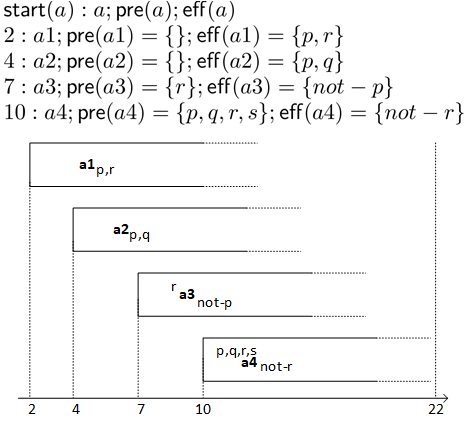
\includegraphics[width=0.75\linewidth]{ejemploacciones3.png}
	\caption{A simple example of how learning the temporal features from $O$ and $A?$ is not straightforward. We (optionally) observe the plan makespan is 22.}
	%, but depending on the distribution of conditions, effects and durations, many situations are possible, though some of them inconsistent.}
	\label{fig:exampleplantrace}
\end{figure}

Let us suppose the example of Fig.~\ref{fig:exampleplantrace}, with observations on the start times, conditions and effects of actions. Clearly, $a3$ needs $a1$ to have $r$ supported, which represents the causal link or dependency $\tup{a1,r,a3}$. Let us imagine that $r$ is in $\cond_s(a3)$. In such a case, if $r$ is in $\eff_s(a1)$, $\dur(a1)$ is irrelevant to $a3$, but if $r$ is in $\eff_e(a1)$, $\dur(a1)$ has to be lower or equal than 5 ($\start(a1)+\dur(a1) \leq \start(a3)$). On the contrary, if $r$ is in $\cond_e(a3)$, $\dur(a1)$ could be much longer. Therefore, the distribution of conditions and effects has a significant impact in the durations, and vice versa.


$a4$ needs $p$, which means two possible causal links ($\tup{a1,p,a4}$ or $\tup{a2,p,a4}$), but 
%The most appropriate causal link will be the last to happen (i.e. the nearest to the requirer), and 
this depends on the effects+durations of $a1$ and $a2$. Therefore, the causal links are unknown, not easy to detect and they affect the structure of the temporal plan. But $a4$ really needs both $a1$ and $a2$ to have $p,q,r$ supported. Let us imagine that $p,q,r$ are in $\cond_s(a4)$ and $p,q$ in $\eff_e(a2)$; then $\dur(a2) \leq 6$. Even if we knew for sure that $\dur(a2)=6$ and $r$ was in $\eff_e(a1)$, we could never estimate the exact value of $\dur(a1)$, as any value in $]0..8]$ would be valid. Intuitively, an action has to wait until the last of its supports, but we cannot grant when the previous supports happen. %; those supporting times and respective durations can never be assured. 
Therefore, in some situations the precise duration cannot be found and we can only provide values that make the model consistent.
An analogous situation would happen if we only observed the end times and all the effects were \textit{at start}.


On the other hand, $a3$ deletes $p$, which means that it might \emph{threat} the causal link $\tup{a1,p,a4}$ or $\tup{a2,p,a4}$. But again, this threat depends on the distribution of conditions+effects and the durations. For instance, if $not-p$ is in $\eff_s(a3)$, then $a1$ or $a2$ must support $p$ after time 7 and before $a4$ requires it, which entails many consistent alternatives. On the contrary, if $p$ is in both $\eff_s(a1)$ and $\eff_s(a2)$, the observations on this plan trace are inconsistent as $a3$ deletes $p$ and no other action in the plan supports $p$ for $a4$ (no solution exists). However, if $not-p$ is in $\eff_e(a3)$, $\dur(a3) > 3$ and $p$ is in $\cond_s(a4)$, then no threat will occur in the plan. Therefore, causal links and threats can easily appear or disappear depending on the selected distributions and durations.

Finally, there are some philosophical questions without a clearly motivated answer. First, why some conditions are modeled as \emph{at start} and others as \emph{over all}? In \texttt{drive-truck} of Fig.~\ref{fig:exampleactions2}, why \texttt{(driving ?d ?t)} is required throughout the entire action but \texttt{(link ?from ?to)} only at its beginning? Apparently, the link between the two locations should remain all over the driving, which is more sensible. So is this a wrong decision of the human modeler? In Fig.~\ref{fig:exampleplantrace}, $s$ is a condition that is not asserted nor deleted in the plan so it can be considered as static information, i.e. invariant (\emph{over all}) knowledge that always holds.\footnote{Static information is commonly used in planning for the grounding process, e.g. to model that there is a link between two locations and, consequently, a driving is possible; to represent that level1 is before level2; to model a petrol station that allows a refuel action in a given location; etc.} 
Second, why some effects are modeled as \emph{at start} and others as \emph{at end}? In \texttt{board-truck}, why is \texttt{(not (empty ?t))} happening \textit{at start} and \texttt{(driving ?d ?t)} \textit{at end}? Could it be in the opposite way? Although this seems sensible here, in some domains it is modeled in the other way round. Third, what happens if one action requires/supports what it deletes (see $a4$ in Fig.~\ref{fig:exampleplantrace}, which might threat itself)? In such a case, the delete effect should happen later than its requirement/supporting.
Four, what happens if all effects are \emph{at start}? This makes little sense, as the duration of the actions would be undetermined and could potentially exceed the known plan horizon or makespan, no matter the problem goals. However, this is possible. In Fig.~\ref{fig:exampleplantrace}, if the effects of $a1$ and $a2$ are \emph{at start}, is it sensible to allow their durations to pass a hypothetical limit of 22? In other words, once all plan goals are achieved, can the actions be executed beyond the plan makespan, or do they need to be cut off to such a value? This could potentially lead to an infinite number of models and overlapping situations. Although infrequent, some humans model durative actions only with start effects, which is a bit irrational. Also, temporally expressive examples with required concurrency~\cite{cushing2007temporal}, where envelope actions are essential to find a plan, significantly increases the number of overlapping situations.

As can be noticed, learning the temporal features is not a simple task whatsoever, and many possible combinations are feasible provided they fit the constraints the problem and observations impose. Therefore, formulating a CSP seems a promising approach to address this learning task.


\section{A CP Formulation to Learn Temporal Features on Action Models}
\label{sec:CPformulation}

Our approach is to create a CSP that includes all the constraints the learning task requires. This includes: i) the observations of start and/or end times; ii) the actions' conditions, effects and durations; iii) the causal structure of the plan with all possible supports; and iv) mechanisms to avoid threats and possible contradictory effects. This formulation is solver-independent. This means that any off-the-shelf CSP solver that supports the expressiveness of our formulation, with binary and non-binary constraints, can be used.


\subsection{Variables}


For each action $a$ in $A?$, we create the seven kinds of variables specified in Table~\ref{table:variables}. Variables define the time-stamps for actions, the causal links, the interval when conditions must hold and the time when the effects happen. For simplicity, and to deal with integer variables, we model time in $\mathbb{Z}^+$. To prevent time from exceeding the plan horizon, we bound all times to the makespan of the plan.\footnote{We use the makespan, which can be observed, to restrict the duration of the actions. However, it is dispensable if we consider a long enough domain for durations.}

	\begin{table*}
	\caption{Formulation of Variables and Their Domains for Actions in $A?$}
	\label{table:variables}
	\begin{center}
		\small
		\begin{tabular}{p{2.2cm}p{3.1cm}p{9.5cm}}
			Variable & Domain & Description \\
			
			\hline
			
			%\multicolumn{3}{l}{Vars. necessary for action times} \\
			
			$\start(a)$ & $[0..makespan]$ & start time of $a$ that might be observed in $O$ or derived\\
			$\dur(a)$ & $[0..makespan]$ & duration of $a$\\
			$\en(a)$ & $[0..makespan]$ & end time of $a$ that might be observed in $O$ or derived \\
			
			%\multicolumn{3}{l}{Vars. necessary for action conditions+effects} \\
			
			$\supp(p,a)$ & $\{b_i\}$ that supports $p$ & symbolic variable for the set of potential supporters $b_i$ of condition $p$ of $a$ (causal link $\tup{b_i,p,a}$) \\
			
			$\reqs(p,a)$, \\
			$\reqe(p,a)$ & $[0..makespan]$ & interval $[\reqs(p,a)..\reqe(p,a)]$ at which action $a$ requires $p$ \\
			
			$\tim(p,a)$ & $[0..makespan]$ & time when effect $p$ of $a$ happens \\
			
			
			\hline
		\end{tabular}
		\normalsize
	\end{center}
\end{table*}




Our temporal model formulation is more expressive than PDDL2.1 (see more details in Section~\ref{sec:PDDL21constraints}), and allows conditions and effects to be at any time, even outside the execution of the action. For instance, let us imagine a condition $p$ that only needs to be maintained for 5 time units before an action $a$ starts (e.g. warming-up a motor before driving): the expression $\reqe(p,a)=\start(a); \reqe(p,a) = \reqs(p,a)+5$ is possible in our formulation. Additionally, we can represent an effect $p$ that happens in the middle of action $a$: $\tim(p,a) = \start(a)+ (\dur(a) / 2)$ is also possible.



Additionally, we create two dummy actions $\ini$ and $\goal$ for each planning problem $\tup{F,I,G,A}$. First, $\ini$ represents the initial state $I$ ($\start(\ini)=0$ and $\dur(\ini)=0$). $\ini$ has no variables $\supp, \reqs$ and $\reqe$ because it has no conditions. $\ini$ has as many $\tim(p_i,\ini)=0$ as $p_i$ in $I$. Second, $\goal$ represents $G$ ($\start(\goal)=makespan$ and $\dur(\goal)=0$). $\goal$ has as many $\supp(p_i,\goal)$ and $\reqs(p_i,\goal)=\reqe(p_i,\goal)=makespan$ as $p_i$ in $G$. $\goal$ has no variables $\tim$ as it has no effects.



This formulation allows us to model TILs
% and observations 
exactly like other actions. $\til(f,t)$ can be seen as a dummy action ($\start(\til(f,t))=t$ and $\dur(\til(f,t))=0$) with no conditions and only one effect $f$ that happens at time $t$ ($\tim(f,\til(f,t))=t$). A $\til$ is similar to $\ini$, as they both represent information that is given at a particular time, but externally to the execution of the plan. 

%On the other hand, $\obs(f,t)$ can be seen as another dummy action ($\start(\obs(f,t))=t$ and $\dur(\obs(f,t))=0$) with only one condition $f$, which is the value observed for fact $f$, and no effects at all. An $\obs$ is analogous to $\goal$, as they both represent conditions that must be satisfied in the execution of the plan at a particular time.


\subsection{Constraints}


Table~\ref{table:constraints} shows the constraints that we define among the variables of Table~\ref{table:variables}. The three first constraints are intuitive enough. The fourth constraint models the causal links. Note that in a causal link $\tup{b_i,p,a}$, $\tim(p,b_i) < \reqs(p,a)$ and not $\leq$. This is because temporal planning assumes an $\epsilon > 0$, as a small tolerance that implies no collision between the time when an effect $p$ is supported and when it is required~\cite{fox2003pddl2}. When time is modeled in $\mathbb{R}^+$, epsilon is usually 0.001 but when it is modeled in $\mathbb{Z}^+$, $\epsilon=1$ and $\leq$ becomes $<$.
The fifth constraint avoids any threat via promotion or demotion~\cite{ghallab2004automated}. The sixth constraint models the fact the same action requires and deletes $p$. Note the $\geq$ inequality here; this is possible because 
%the underlying semantics in planning considers that if conditions and effects of the same action happen at the same time, the conditions are always checked instantly before the effects
if one condition and one effect of the same action $a$ happen at the same time, the underlying semantics in planning considers the condition in $a$ is checked instantly before the effect in $a$~\cite{fox2003pddl2}. The seventh constraint solves the fact that two (possibly equal) actions have contradictory effects. 

It is important to note that the constraints involve any type of actions. Consequently, $\ini$, $\goal$ and $\til$ are subsumed in this formulation.


\begin{table*}
	\caption{Formulation of Constraints.}
	\label{table:constraints}
	\begin{center}
		\small
		\begin{tabular}{p{5cm}p{11cm}}
			Constraint & Description \\
			
			\hline
			
			$\en(a)=\start(a)+\dur(a)$ & relation between start and end time of $a$ \\
			
			$\en(a) \leq \start(\goal)$ & $\goal$ is always the last action of the plan \\
			
			%$\reqs(p,a) \leq \reqe(p,a)$ & [$\reqs(p,a)..\reqe(p,a)$] must be a valid interval \\
			$\reqs(p,a) \leq \reqe(p,a)$ & interval [$\reqs(p,a)..\reqe(p,a)$] must be a valid interval \\
			
			\begin{tabular}{l}
				\hspace{-0.2cm}if $\supp(p,a)=b_i$ then \\
				$\tim(p,b_i) < \reqs(p,a)$
			\end{tabular}
			& modeling causal link $\tup{b_i,p,a}$: the time when $b_i$ supports $p$ must be before $a$ requires $p$ \\
			
			\begin{tabular}{l}
				\hspace{-0.2cm}$\forall b_j \neq a$ that deletes $p$ at time $\tau_j$: \\
				if $\supp(p,a)=b_i$ then \\
				\hspace{0.2cm}$\tau_j < \tim(p,b_i)$ OR \\
				\hspace{0.2cm}$\tau_j > \reqe(p,a)$
			\end{tabular}
			& solving threat of $b_j$ to causal link $\tup{b_i,p,a}$ being $b_j \neq a$ (promotion OR demotion)\\
			
			\begin{tabular}{l}
				\hspace{-0.2cm}if $a$ requires and deletes $p$: \\
				$\tim(not-p,a) \geq \reqe(p,a)$ \\
			\end{tabular}
			& when $a$ requires and deletes $p$, the effect cannot happen before the condition \\
			
			\begin{tabular}{l}
				\hspace{-0.2cm}$\forall a_i,a_j \mid a_i$ supports $p$ and \\
				\hspace{1cm}$a_j$ deletes $p$: \\
				$\tim(p,a_i) \neq \tim(not-p,a_j)$ \\
			\end{tabular}
			& solving effect interference ($p$ and $not-p$): they cannot happen at the same time \\
			
			\hline
		\end{tabular}
		\normalsize
	\end{center}
\end{table*}



\subsection{Specific Constraints for Durative Actions of PDDL2.1}
\label{sec:PDDL21constraints}

As Section~\ref{sec:temporalplanning} explains, PDDL2.1 restricts the expressiveness of temporal planning in terms of conditions, effects, durations and structure of the actions. Hence, our temporal formulation subsumes and is significantly richer than PDDL2.1; but adding constraints to make it fully PDDL2.1-compliant is straightforward.


First, adding $((\reqs(p,a) = \start(a))$ OR ($\reqs(p,a) = \en(a)))$ AND $((\reqe(p,a) = \start(a))$ OR ($\reqe(p,a) = \en(a)))$ limits condition $p$ to be \emph{at start}, \emph{over all} or \emph{at end}, i.e. $p$ is in $\cond_s(a)$, $\cond_o(a)$ or $\cond_e(a)$, respectively.
Further, if a condition $p$ is never deleted in a plan, it can be considered as static or invariant information, and 
the constraint to be added is simply: $((\reqs(p,a) = \start(a))$ AND $(\reqe(p,a) = \en(a)))$, i.e. $p \in \cond_o(a)$.
Surprisingly, invariant conditions are modeled differently depending on the human modeler. See, for instance, \texttt{(link ?from ?to)} of Fig.~\ref{fig:exampleactions2}, which is modeled as an \emph{at start} condition despite: i) the link should be necessary all over the driving; and ii) no action in this domain deletes that link.
This also happens in the \emph{transport} domain of the IPC, where a \texttt{refuel} action requires to have a petrol station in a location only \emph{at start}, rather than \emph{over all} which makes more sense. This shows that modeling the temporal features is not easy even for an expert and it highly depends on the human's decision. On the contrary, our formulation checks the invariant conditions and deals with them always in the same coherent way.


Second, $((\tim(p,a) = \start(a))$ OR $(\tim(p,a) = \en(a)))$ makes an effect $p$ happen only \emph{at start} or \emph{at end} of action $a$, i.e. $p$ is in $\eff_s(a)$ or $\eff_e(a)$.
Also, if all effects happen \emph{at start} the duration of the action would be irrelevant and could exceed the plan makespan. To avoid this, for any action $a$, at least one of its effects should happen \emph{at end}: $\sum_{i=1}^{n =|\eff(a)|} \tim(p_i,a) > n \times \start(a)$, which guarantees $\eff_e(a)$ is not empty.

%\begin{displaymath}
%\sum_{i=1}^{n = \textrm{number of effects of }a} \tim(p_i,a) > n \times \start(a)
%\end{displaymath}


Third, durations in PDDL2.1 can be defined in two different ways. On the one hand, durations can be equal for all grounded actions of the same operator. For instance, any instantiation of \texttt{board-truck} of Fig.~\ref{fig:exampleactions2} will last 2 time units no matter its parameters. Although this may seem a bit odd, it is not an uncommon practice to simplify the model. The constraint to model this is: $\forall a_i,a_j$ being instances of the same operator: $\dur(a_i) = \dur(a_j)$.
On the other hand, although different instantiations of \texttt{drive-truck} will last different depending on the locations, different occurrences of the same instantiated action will last equal.
In a PDDL2.1 temporal plan, multiple occurrences of \texttt{drive-truck(truck1,loc1,loc2,driver1)} will have the same duration no matter when they start. Intuitively, they are different occurrences of the same action, but in the real-world the durations would differ from driving at night or in peak times. Since PDDL2.1 makes no distinction among different occurrences, the constraint to add is: $\forall a_i,a_j$ being occurrences of the same durative action: $\dur(a_i) = \dur(a_j)$.
Obviously, this second constraint is subsumed by the first one in the general case where all instances of the same operator have the same duration.

Fourth, the structure of conditions and effects for all grounded actions of the same operator is constant in PDDL2.1. This means that if \texttt{(empty ?t)} is an \emph{at start} condition of \texttt{board-truck}, it will be \emph{at start} in any of its grounded actions.
Let $\{p_i\}$ be the conditions of an operator and $\{a_j\}$ be the instances of a particular operator. The following constraints are necessary to guarantee a constant structure:

$\forall p_i: (\forall a_j: \reqs(p_i,a_j) = \start(a_j))$ OR $(\forall a_j: \reqs(p_i,a_j) = \en(a_j))$

$\forall p_i: (\forall a_j: \reqe(p_i,a_j) = \start(a_j))$ OR $(\forall a_j: \reqe(p_i,a_j) = \en(a_j))$

And analogously for all effects $\{p_i\}$ and the instances $\{a_j\}$ of an operator:

$\forall p_i: (\forall a_j: \tim(p_i,a_j) = \start(a_j))$ OR $(\forall a_j: \tim(p_i,a_j) = \en(a_j))$


As a conclusion, in our formulation each action of $A?$ is modeled separately so it does not need to share the same structure or duration of other actions. Moreover, the time-stamps for conditions/effects can be arbitrarily placed inside or outside the execution of the action, which allows for a flexible and expressive temporal model. But, when necessary, we can simply include additional constraints to restrict the expressiveness of the model, such as the ones provided by PDDL2.1, because the operator is directly extracted from the action's name.


\subsection{Example}
\label{sec:example}

We now show a fragment of the formulation for the example depicted in Fig.~\ref{fig:exampleplantrace}. For simplicity, we only show the variables and constraints for action $a3$, but the formulation is analogous for all other actions.

The variables and domains are: $\start(a3)=7$; $\dur(a3) \in [1..15]$; $\en(a3)=\start(a3)+\dur(a3)$; $\supp(r,a3) \in \{a1\}$; $\reqs(r,a3),\reqe(r,a3) \in [0..22]$; and $\tim(not-p,a3) \in [0..22]$.
On the other hand, the constraints are: $\en(a3) \leq \start(\goal)$; $\reqs(r,a3) \leq \reqe(r,a3)$; if $\supp(r,a3)=a1$ then $\tim(r,a1) < \reqs(r,a3)$; if $\supp(r,a3)=a1$ then $((\tim(not-r,a4) < \tim(r,a1))$ OR $(\tim(not-r,a4) > \reqe(r,a3)))$; $\tim(not-p,a3) \neq \tim(p,a1)$ and $\tim(not-p,a3) \neq \tim(p,a2)$.


There is an unaffordable number of solutions to this simple example, mainly because there is a huge range of possible durations that make the learned model consistent with the partially specified model $A?$. A solution has assigned consistent values to all variables of Table~\ref{table:variables} and satisfies all the constraints of Table~\ref{table:constraints} for this example.
Fig.~\ref{figure:solutionsExample} shows six solution models, randomly chosen from the first 100 solutions. What is important to note is that the structure, i.e. distribution of conditions/effects, is similar in all the learned models. Actually, the distribution of the effects is identical (except for $q$ in model 2), and the distribution of conditions is very similar (e.g. $q$ is always in $\cond_o$ and $r$ in $a4$ is very often in $\cond_o$). Obviously, learned models tend to be similar, which is very positive. Indiscriminately changing a single feature means a different, though similar, learned model that might fail to satisfy the constraints and lead to an inconsistency.
%This shows that the one-shot learning returns not only consistent models but also similar, which is very positive.
The durations are, however, more different: $\dur(a1)$ ranges in these models from 7 to 19, whereas $\dur(a2)$ ranges from 5 to 18. As explained in Section~\ref{sec:simpleTask}, learning the precise duration from just one sample may not be always possible, which is the main limitation of the one-shot learning task.
%Clearly, the duration learned for only one sample of \texttt{drive-truck(truck1,loc1,loc2,driver1)} cannot be always generalized to any other driving between these two locations.
In fact, the specific constraint of PDDL2.1, with regard to having multiple occurrences of the same action having the same duration, can significantly help us to learn the actions' duration in a more precise way, because the learned duration must be consistent with all those occurrences.


\begin{figure*}
	\center
	{\footnotesize 
	\begin{tabular}{ll}
		\hspace{-0.6cm}\begin{tabular}{lllllll}
			Action & $\dur$ & $\cond_s$ & $\cond_o$ & $\cond_e$ & $\eff_s$ & $\eff_e$ \\
			
			\hline
			
			\multicolumn{7}{l}{Learned model 1} \\
			$a1$ & 8 & & & & $r$ & $p$ \\
			$a2$ & 18 & & & & $q$ & $p$ \\
			$a3$ & 1 & & $r$ & & & $not-p$ \\
			$a4$ & 1 & & $q,r$ & $p$ & & $not-r$ \\
			
			\hline
			
			\multicolumn{7}{l}{Learned model 2} \\
			$a1$ & 19 & & & & $r$ & $p$ \\
			$a2$ & 5 & & & & & $p,q$ \\
			$a3$ & 1 & & & $r$ & & $not-p$ \\
			$a4$ & 1 & $r$ & $p,q$ & & & $not-r$ \\
			
			\hline
			
			\multicolumn{7}{l}{Learned model 3} \\
			$a1$ & 7 & & & & $r$ & $p$ \\
			$a2$ & 18 & & & & $q$ & $p$ \\
			$a3$ & 1 & & & $r$  & & $not-p$ \\
			$a4$ & 1 & & $p,q,r$ & & & $not-r$ \\
		\end{tabular} &
		
		\hspace{0.3cm}\begin{tabular}{lllllll}
			
			Action & $\dur$ & $\cond_s$ & $\cond_o$ & $\cond_e$ & $\eff_s$ & $\eff_e$ \\
			
			\hline
			
			\multicolumn{7}{l}{Learned model 4} \\
			$a1$ & 7 & & & & $r$ & $p$ \\
			$a2$ & 9 & & & & $q$ & $p$ \\
			$a3$ & 1 & & & $r$ & & $not-p$ \\
			$a4$ & 1 & & $p,q,r$ & & & $not-r$ \\
			
			\hline
			
			\multicolumn{7}{l}{Learned model 5} \\
			$a1$ & 9 & & & & $r$ & $p$ \\
			$a2$ & 6 & & & & $q$ & $p$ \\
			$a3$ & 1 & & $r$ & & & $not-p$ \\
			$a4$ & 1 & & $q,r$ & $p$ & & $not-r$ \\
			
			\hline
			
			\multicolumn{7}{l}{Learned model 6} \\
			$a1$ & 8 & & & & $r$ & $p$ \\
			$a2$ & 16 & & & & $q$ & $p$ \\
			$a3$ & 1 & $r$ & & & & $not-p$ \\
			$a4$ & 1 & & $q,r$ & $p$ & & $not-r$ \\
			
		\end{tabular} \\
		
	\end{tabular}
	}
	
	\caption{Six learned models, randomly chosen from the first 100 solutions, to the example of Fig.~\ref{fig:exampleplantrace}.}
	\label{figure:solutionsExample}
\end{figure*}


%\subsection{Properties}

%Soundness of our formulation is guaranteed by the definition of the constraints of Table~\ref{table:constraints}, where all the branching alternatives to solve causal links, threats and effect interferences are supported. Completeness is guaranteed by the complete exploration of the domain of each variable of Table~\ref{table:variables} which can return many learned models in the form of consistent alternative solutions.



\subsection{Implementation. Use of Heuristics for Resolution}
\label{sec:implementation}

Our CSP formulation is automatically compiled from a partially specified action model, as defined in a classical planning problem, and the observations from a plan execution.
The formulation has been implemented in \textsf{Choco}\footnote{\textsf{Choco} is available at \texttt{www.choco-solver.org}}, an open-source Java library for CP that provides an object-oriented API to state the constraints to be satisfied.

Our formulation is solver-independent, which means we do not use heuristics that may require changes in the implementation of the CSP engine.
Although this reduces the solver's performance, we are mainly interested in using it as a blackbox that can be easily changed with no modification in our formulation. However, we can easily encode standard static heuristics for variable and value selection that help improve efficiency by following the next ordering, which has shown very efficient in our experiments:

%%IMPORTANTE: ahorramos espacio juntando en la viñeta el orden de seleccion de variables y de valores

%From the variable perspective, we have detected it is better to instantiate variables that first lead to failure: effects, conditions, supporters and durations. This implies this ordering: $\tim$, $\reqs$, $\reqe$, $\supp$ and $\dur$.
%From the value perspective, we select first the values that lead to a more reasonable model of actions:

\begin{enumerate}
	\item Effects ($\tim$). For negative effects, first the lower value and for positive effects, first the upper value. This gives priority to delete effects as $\eff_s(a)$ and positive effects as $\eff_e(a)$.
	\item Conditions ($\reqs$ and $\reqe$). For $\reqs$, first the lower value, whereas for $\reqe$, first the upper value. This gives priority to $\cond_o(a)$, trying to keep the conditions as long as possible.
	\item Supporters ($\supp$). First the lower value, thus preferring the supporter that starts earlier in the plan.
	\item Duration ($\dur$). First the lower value, thus applying the principle of the shortest actions that make the learned model consistent.
\end{enumerate}


%This simple collection of heuristics is very intuitive and has been used in \textsf{Choco} by simply overriding the default search strategy for the variable and value selectors. Although these heuristics have shown very efficient in our experiments, they cannot always guarantee the best performance.


\subsection{Using the CP Formulation for Plan Validation}
\label{sec:usingCPValidation}

%As seen above, adding constraints allows us to restrict the temporal expressiveness of the learned model.
We explained that adding extra constraints allows us to restrict the temporal expressiveness of the learned model. We show here that we can also restrict the learned model by constraining the variables to known values, which is specially interesting when there is additional information on the temporal model that needs to be represented. For instance, based on past learned models, we may know the precise duration of an action $a$ is 6,
%or we can figure out that a condition is a start condition
or we can figure out that its effect $p$ always happens at end.
Our CP formulation can include this by simply adding $\dur(a)=6$ and $\tim(p,a)=\en(a)$, respectively, which is useful to enrich the partially specified actions in $A?$ of the learning task.

%The CP formulation is also useful to validate whether a given action model is consistent, as we will see in Section~\ref{sec:evaluation}.
In particular, the possibility of adding those constraints is very appealing when used for validating whether a partial action model allows us to learn a consistent model, as we will see in Section~\ref{sec:evaluation}. This leads us to a unified formulation for learning and validation.
Let us assume that the distribution of all (or just a few) conditions and/or effects is known and, in consequence, represented in the learning task. If a solution is found, then that structure of conditions/effects is consistent for the learned model. On the contrary, if no solution is found that structure is inconsistent and cannot be explained.
Analogously, we can represent known values for the durations. If a solution is found, the durations are consistent, and inconsistent otherwise.
Hence, we have three options for validating a partial model \emph{w.r.t.}: i) a known structure with the distribution of conditions/effects; ii) a known set of durations; and iii) a known structure plus a known set of durations (i+ii).
The first and second option allows for some flexibility in the learning task because some variables remain open. On the contrary, the third option checks whether a learned model can fit the given constraints, thus reproducing a plan validation task equivalent to~\cite{howey2004val}, but now much more expressive.



\section{Evaluation}
\label{sec:evaluation}


This section evaluates our approach from two points of view. First, we assess the performance of the CP formulation for solving the learning task.
Second, we assess the quality of the resulting learned model.
 
 
\subsection{Setup}

We have run 569 different instances, from the simplest to the most complex ones, on nine IPC planning domains. These domains are encoded in PDDL2.1, so we have included the constraints given in Section~\ref{sec:PDDL21constraints}. We first get the plans for these domains by using five planners (\textit{LPG-Quality}~\cite{gerevini2003planning}, \textit{LPG-Speed}~\cite{gerevini2003planning}, \textit{TP}~\cite{jimenez2015temporal}, \textit{TFD}~\cite{eyerich2009using} and \textit{TFLAP}~\cite{marzal2016temporal}), where the planning time is limited to 100s.
The actions and their start time observations on each plan are automatically compiled into a CSP learning instance. Then,
%we create the CP formulation and
we run the one-shot learning task to get the action model (with the temporal features) for each instance, where the learning time is limited to 100s on an Intel i5-6400 @ 2.70GHz with 8GB of RAM. Since each CSP instance can have many solutions, we always select the first solution found.



\subsection{Performance Evaluation}

We measure the performance of the learning task in terms of the size of the CP formulation, according to the variables and constraints defined in Section~\ref{sec:CPformulation}. Table~\ref{table:formulationdetails} shows the number of instances tested per domain, and the min-max (and average between brackets) number of variables and constraints of the formulation for all the instances. The last column shows the average resolution time per instance.
For example, the \emph{zenotravel} domain contains 78 instances, which means compiling 78 formulations. The formulations' size ranges from 98 to 2878 variables and from 352 to 56402 constraints. The average resolution time per formulation is 0.02s.

In all the domains, the number of variables is high, but since they are highly constrained the resolution time remains very low.
This is a consequence of the one-shot learning approach, which only needs to include the variables+constraints of one plan instance, thus requiring less computation time.


\begin{table*}
	\caption{CP Formulation Details for the Instances of IPC Domains.}
	\label{table:formulationdetails}
	\begin{center}
		\small
		%\begin{tabular}{p{2cm}p{2cm}p{1cm}p{1cm}}
		\begin{tabular}{p{1.3cm}cccc}
			Domain & \#instances & \#variables (average) & \#constraints (average) & average resolution time (s)   \\
			
			\hline
			
			\emph{zenotravel} & 78 & 98-2878 (825) & 352-56402 (8520) & 0.02 \\
			\emph{driverlog} & 73 & 193-14043 (2862) & 847-170146 (18457) & 0.08 \\
			\emph{depots} & 64 & 242-2943 (1142) & 1577-430688 (20318) & 0.04 \\
			\emph{rovers} & 84 & 290-9307 (1991) & 1010-48501 (10540) & 0.20 \\
			\emph{satellite} & 84 & 174-3054 (1189) & 967-19709 (6294) & 0.05 \\
			\emph{storage} & 69 & 99-3479 (704) & 3023-597178 (17213) & 0.03 \\
			\emph{floortile} & 17 & 2564-7994 (4647) & 14073-847609 (129881) & 0.20 \\			
			\emph{parking} & 49 & 539-1275 (834) & 2581-7366 (4208) & 0.03 \\
			\emph{sokoban} & 51 & 8586-57779 (21142) & 35882-390316 (97133) & 0.44 \\
			
			\hline
		\end{tabular}
		\normalsize
	\end{center}
\end{table*}



\subsection{Quality Evaluation}

The quality evaluation of the learned model can be addressed from two perspectives. From a pure syntactic perspective, learning can be considered as an automated design task to create a new model that is similar to a reference (or {\em ground truth}) model. The aim is to assess the precision or accuracy of the learned model, a common metric in learning~\cite{aineto2018icaps,Zhuo2014,ZhuoYHL10}.
From a semantic perspective, learning can be considered as a classification task, where we first learn a model from a training dataset and then validate it on a test dataset. The aim is to assess how much the learned model explains (or transfers) to unseen test samples~\cite{Aggarwal2016,Jialin2010,ZhuoQ14}.


\subsubsection{Syntactic Evaluation. Precision}


Precision in learning is a similarity measure between two models, one reference and one learned model. In our case, $precision=100 \times \frac{f^{=}}{f^{=} + f^{\neq}}$, where $f^{=}$ counts the number of facts (i.e. conditions+effects) that are temporally distributed equally in both models, and $f^{\neq}$ counts the number of facts that are distributed in a different way. 
As an example, given an action or operator, if $p$ is an \textit{at start} condition in the reference model and also in the learned model, it counts as a hit in $f^{=}$, and in $f^{\neq}$ if they differ. This is repeated for all conditions and effects. A precision of 100\% means the \texttt{:condition} and \texttt{:effect} sections in both models are, respectively, syntactically identical. Roughly speaking, the learned structure of conditions/effects matches exactly the reference model.

Table~\ref{table:precisonevaluation} shows the syntactic evaluation for our 569 learned models, including the number of operators (or action schemas), the total number of facts ($f^{=}+f^{\neq}$) to distribute within the operators, and the average precision scores. We first use as the reference model the hand-written domain as provided in IPC.
On average, the precision scores are very good, taking into consideration that the learning is done under a one-shot approach. The ratios range from 49.63\% in \textit{rovers}, the domain with the highest number of operators and facts, to 97.80\% for \textit{sokoban}, the domain with the lowest number of operators.



\begin{table}
	\caption{Precision \textit{w.r.t.} a REFerence and a More Rational REVised Model.}
	\label{table:precisonevaluation}
	\begin{center}
		\small
		%\begin{tabular}{p{2cm}p{2cm}p{1cm}p{1cm}}
		\begin{tabular}{p{1.3cm}cccc}
			Domain & \#ops & \#facts & REF model & REV model  \\
			
			\hline
			
			\emph{zenotravel} & 5 & 28 & 61.04\% & 83.99\% \\
			\emph{driverlog} & 6 & 28 & 76.52\% & 83.71\% \\
			\emph{depots} & 5 & 37 & 74.66\% & 75.25\% \\
			\emph{rovers} & 9 & 69 & 49.63\% & 84.64\% \\
			\emph{satellite} & 5 & 24 & 71.72\% & 71.72\% \\
			\emph{storage} & 5 & 38 & 80.99\% & 81.37\% \\
			\emph{floortile} & 7 & 44 & 81.42\% & 81.42\% \\			
			\emph{parking} & 4 & 31 & 77.46\% & 77.46\% \\
			\emph{sokoban} & 3 & 33 & 97.80\% & 97.80\% \\
			
			\hline
		\end{tabular}
		\normalsize
	\end{center}
\end{table}


Unfortunately, there is not a unique reference model when learning real-world temporal models; e.g. \texttt{full} and \texttt{not-empty} effects can be interchangeable in some domains, as they represent the same information, but they are syntactically different.
Also, a pure syntax-based measure may return misleading results, as it may count as incorrect ($f^{\neq}$) a change in the distribution of conditions/effects that represents an equivalent reformulation of the reference model. For instance, given the example of Fig.~\ref{fig:exampleactions2}, the condition learned \texttt{(over all (link ?from ?to))} would be counted as a difference for action \texttt{drive-truck}, as it is \textit{at start} in the reference model; but it is, rationally speaking, even more correct. 
This misleading situation is common in IPC, where the domains' definition is not always rational due to: i) \textit{at start} conditions that should be \textit{over all} (in \emph{zenotravel}, \emph{driverlog} and \emph{rovers}); ii) \textit{at start} effects that should be \textit{at end}, and vice versa (in \emph{zenotravel}, \emph{depots}, \emph{rovers} and \emph{satellite}); and iii) actions with only \textit{at start} effects that make durative actions unnecessarily tricky (in \emph{depots}).
As a knowledge engineering step, we have revised all the domains to make them more rational and recalculated the precision. The results are shown in the last column of Table~\ref{table:precisonevaluation}.
Learned models are significantly more precise in the revised domains (specially in \emph{zenotravel} and \textit{rovers}), ranging now from 71.72\% to 97.80\%. 
This means the \texttt{:condition} and \texttt{:effect} sections are, respectively, syntactically identical in more than 70\% of the revised \textit{vs.} learned models.
Also, 100\% of the \textit{over all} conditions that represent static information is precisely learned, thus being more coherent than human designers.
In \emph{satellite} however, the results remain the same, as the learned models still mislead some inner effects within the actions.
Obviously, the reference domains that are well defined and need no revision (\emph{floortile}, \emph{parking} and \emph{sokoban}) return the same precision scores.




\subsubsection{Semantic Evaluation. Explanation and Validation}

As pointed out above, the temporal ground truth about the temporal world is not unique. A precision score of 75\% might still be an excellent result, provided the learned model explains all the observations of the plan trace; that is, the model is consistent because it satisfies all the constraints of the learning task.
Also, as seen in Section~\ref{sec:simpleTask}, some learned durations cannot be granted and will differ from a reference model, but the underlying model is still consistent.
For instance, the six learned models of Fig.~\ref{figure:solutionsExample} are not syntactically identical, but they are all consistent for the example of Fig.~\ref{fig:exampleplantrace}. 
Therefore, a syntactic evaluation in learning is a bit limited and we should perform a further semantic evaluation. From this standpoint, the quality of the learned model can be assessed by analyzing the success ratio of the learned model \emph{vs.} unseen samples of a test dataset, analogously to a classification task. 
We define the success ratio as $success=100 \times \frac{samples^{\checkmark}}{|dataset|}$, where $samples^{\checkmark}$ counts the number of samples the learned model explains on a test $dataset$. A success of 100\% implies learning a model that explains the full dataset: a feasible solution is found which is consistent with the constraints of the learned model together with the test samples ones. 
But if, for example, one condition is learned as \textit{at start} but it leads to an inconsistency in a test sample (where it must remain \textit{over all}), this does not count in $samples^{\checkmark}$.


Given the learned model for an instance of a domain, we assess the quality of such a model \textit{vs.} a dataset formed by the remaining instances of that domain.
For example, the \emph{zenotravel} domain contains 78 instances, as indicated in Table~\ref{table:formulationdetails}, which means learning 78 models. Each model is evaluated by using the 77 remaining models, thus producing 78$\times$77=6006 tests. Each test is repeated three times to validate each model \emph{vs.} the other models \emph{w.r.t.} the \emph{struct}ure, the \emph{dur}ation and the \emph{struct}ure+\emph{dur}ation, as discussed in Section~\ref{sec:usingCPValidation}.
Table~\ref{table:evaluationExperiments} shows the average success ratio for our IPC domains.


In \emph{zenotravel}, the struct value means that the distribution of conditions/effects learned by using only one plan sample is consistent with all the samples used as dataset (100\% of the 6006 tests), which is the perfect result, as also happens in \emph{floortile} and \emph{sokoban} domains.
The dur value means the durations learned explain 68.83\% of the dataset. This value is usually lower because any learned duration that leads to inconsistency in a sample counts as a failure. The struct+dur value means that the learned model explains entirely 35.76\% of the samples. This value is always the lowest because a subtle change in the structure or duration learned that leads to inconsistency counts as a failure. The results depend on the domain size (number of operators, which need to be grounded), the relationships (causal links, threats and interferences) among the actions, and the size and quality of the plans.
The worst result is returned in the \emph{rovers} domain, which models a group of planetary rovers to explore the planet they are on. Since there are many facts, parallel actions for taking pictures/samples and navigation of multiple rovers, learning the duration and the structure+duration is particularly complex in this domain.


In general, the quality of the learned models is good enough to explain a significant number of test samples, specially in terms of the structure. This is interesting, taking into consideration that the one-shot approach uses only one sample to learn the temporal features. However, learning the durations proves more complex. In some cases, we have observed that planners return plans with unnecessary actions, which has a negative impact for learning precise durations, as happens in \emph{rovers}.


\begin{table}
	\caption{Average Success of the One-shot Learned Model \emph{vs.} the Test Dataset.}
	\label{table:evaluationExperiments}
	\begin{center}
		\small
		%\begin{tabular}{p{2cm}pp{1cm}p{1cm}p{2cm}}
		\begin{tabular}{p{1.3cm}cccc}
			Domain & \#tests & struct & dur & struct+dur  \\
			
			\hline
			
			\emph{zenotravel} & 6006 & 100\% & 68.83\% & 35.76\% \\
			\emph{driverlog} & 5256 & 97.60\% & 44.86\% & 21.04\% \\
			\emph{depots} & 4032 & 55.41\% & 76.22\% & 23.19\% \\
			\emph{rovers} & 6972 & 78.84\% & 5.35\% & 0.17\% \\
			\emph{satellite} & 6972 & 80.74\% & 57.13\% & 40.53\% \\
			\emph{storage} & 4692 & 58.08\% & 70.10\% & 38.36\% \\
			\emph{floortile} & 272 & 100\% & 80.88\% & 48.90\%\\			
			\emph{parking} & 2352 & 86.69\% & 81.38\% & 54.89\% \\
			\emph{sokoban} & 2550 & 100\% & 87.25\% & 79.96\% \\
			
			\hline
		\end{tabular}
		\normalsize
	\end{center}
\end{table}




%\section{Discussion}
%\label{sec:discussion}

%Indicar que cambios hace falta para que un cp-planner pueda actuar como learner/validator.


\section{Conclusions}
\label{sec:conclusions}


%Learning in planning is specially interesting to recognize past behavior in order to predict and anticipate actions to improve decisions.
The interest in learning is growing up because it allows us to acquire procedural knowledge through demonstration and partial observations.
% of users' behavior. 
Learning planning action models by observations of plan traces is useful in many scenarios: recognition of past behavior for prediction and anticipation, decision taking and recommendation, programming and modeling, teleoperation, macro recording, sensing and controlling, robotics motion capturing and planning, etc. %(see~\cite{Lauretti2018})
Learning is appealing because these scenarios include a huge number of tasks, sometimes difficult to be described formally (and more difficult to be annotated temporally), which require expert knowledge and engineering that becomes impractical in complex domains.

In this paper we have presented a purely declarative CP formulation, independent of any CSP solver, to address the automated learning of temporal features on action models which, to our knowledge, initiates a novel approach for the intersection of knowledge engineering, learning, CP and planning. Metaphorically speaking, learning the classical model is to planning what learning the temporal features is to temporal planning. Knowing these features is useful in practice, where learning a classical planning model is not enough and needs to be extended with temporal features to 
%be more realistic and 
increase its applicability.
In consequence, learning the temporal features bridges the gap between the planning action model and the real (temporal) world.


%Our main result is a simple formulation that is automatically derived from the actions and observations on each plan execution
Our main result is an effective formulation that is automatically derived, without the necessity of specific hand-coded domain knowledge. The ultimate goal of this learning is to reduce the laborious modeling stage, to minimize the effort human experts need to design temporal planning models before launching the planners. Our formulation is flexible enough to accommodate different types of observations as input information/knowledge, and 
supports a rich temporal planning model with concurrency; although its expressiveness is beyond PDDL2.1, it can be easily modified to be PDDL2.1-compliant.
Formal properties are inherited from the formulation itself and the CSP solver. The formulation is correct because the definition of constraints to solve causal links, threats and effect interferences are supported, which avoids contradictions. It is also complete because the solution needs to be consistent with all the imposed constraints, while a complete exploration of the domain of each variable returns all the possible learned models in the form of alternative consistent solutions.



Unlike other approaches that need to learn from datasets with many samples, we perform a one-shot learning task. Large datasets could lead to better learned models but: i) retrieving many samples is not always easy, specially in human interactive environments that require learning by demonstration; and ii) this would need to estimate the best number of samples and to learn a model that explains the highest number of samples, involving an optimization process, more expensive than satisfaction. Our approach reduces both the size of the required datasets and the computation time. Note, however, that we can easily deal with a large number of input samples by simply including more input observations in our learning task, i.e. by using very long plan traces. And this requires no changes in our CP formulation.

According to our syntactic+semantic evaluation, the one-shot learned models are precise and explain a high number of samples in the datasets used for testing. Moreover, the same CP formulation is valid for learning and for validation, by simply adding constraints to the variables. This is an innovative advantage, as the same formulation allows us to carry out different tasks: from entirely learning, partial learning/validation (structure and/or duration) to entirely plan validation.
From our experiments, learning the structure of the actions in a one-shot way leads to representative enough models, but learning the precise durations is more difficult when irrelevant actions are planned.



Finally, it is important to note that our CP formulation can be represented and solved by Satisfiability Modulo Theories, which is part of our current work. As for future work, we want to extend our formulation to learn from intermediate observations (we need to investigate how many and how frequent they must be), to learn meta-models (as combinations of several learned models), and to learn more complete action models.
In the latter, we will relax the input action model to find out the conditions/effects together with their temporal distribution.
This implies to remove constraints from the partially specified set of actions in $A?$ and to investigate the dependencies between the conditions/effects and temporal features (e.g. some effects could conditionally happen depending on temporal constraints).
The underlying idea of finding an action model consistent with all the constraints will remain exactly the same, but the model will need to be extended with additional decision variables ($\mathsf{is\_condition}(p,a)$ and $\mathsf{is\_effect}(p,a)$) and constraints to decide whether $p$ is a condition or effect of action $a$. This will provide a very open model of actions (we will need to investigate whether the learned model is still precise and valid) that will lead to the analysis of new heuristics for its resolution.



% use section* for acknowledgment
%\ifCLASSOPTIONcompsoc
%  % The Computer Society usually uses the plural form
%  \section*{Acknowledgments}
%\else
%  % regular IEEE prefers the singular form
%  \section*{Acknowledgment}
%\fi


%The authors would like to thank...


% Can use something like this to put references on a page
% by themselves when using endfloat and the captionsoff option.
\ifCLASSOPTIONcaptionsoff
  \newpage
\fi



% trigger a \newpage just before the given reference
% number - used to balance the columns on the last page
% adjust value as needed - may need to be readjusted if
% the document is modified later
%\IEEEtriggeratref{8}
% The "triggered" command can be changed if desired:
%\IEEEtriggercmd{\enlargethispage{-5in}}

% references section

% can use a bibliography generated by BibTeX as a .bbl file
% BibTeX documentation can be easily obtained at:
% http://mirror.ctan.org/biblio/bibtex/contrib/doc/
% The IEEEtran BibTeX style support page is at:
% http://www.michaelshell.org/tex/ieeetran/bibtex/
%\bibliographystyle{IEEEtran}
% argument is your BibTeX string definitions and bibliography database(s)
%\bibliography{IEEEabrv,../bib/paper}
%
% <OR> manually copy in the resultant .bbl file
% set second argument of \begin to the number of references
% (used to reserve space for the reference number labels box)
\bibliographystyle{IEEEtran}
\bibliography{tmodeling}

%\begin{thebibliography}{1}
%\end{thebibliography}

% biography section
% 
% If you have an EPS/PDF photo (graphicx package needed) extra braces are
% needed around the contents of the optional argument to biography to prevent
% the LaTeX parser from getting confused when it sees the complicated
% \includegraphics command within an optional argument. (You could create
% your own custom macro containing the \includegraphics command to make things
% simpler here.)
%\begin{IEEEbiography}[{\includegraphics[width=1in,height=1.25in,clip,keepaspectratio]{mshell}}]{Michael Shell}
% or if you just want to reserve a space for a photo:

%\begin{IEEEbiography}{Michael Shell}
%Biography text here.
%\end{IEEEbiography}
%
%% if you will not have a photo at all:
%\begin{IEEEbiographynophoto}{John Doe}
%Biography text here.
%\end{IEEEbiographynophoto}

% insert where needed to balance the two columns on the last page with
% biographies
%\newpage

\end{document}



% An example of a floating figure using the graphicx package.
% Note that \label must occur AFTER (or within) \caption.
% For figures, \caption should occur after the \includegraphics.
% Note that IEEEtran v1.7 and later has special internal code that
% is designed to preserve the operation of \label within \caption
% even when the captionsoff option is in effect. However, because
% of issues like this, it may be the safest practice to put all your
% \label just after \caption rather than within \caption{}.
%
% Reminder: the "draftcls" or "draftclsnofoot", not "draft", class
% option should be used if it is desired that the figures are to be
% displayed while in draft mode.
%
%\begin{figure}[!t]
%\centering
%\includegraphics[width=2.5in]{myfigure}
% where an .eps filename suffix will be assumed under latex, 
% and a .pdf suffix will be assumed for pdflatex; or what has been declared
% via \DeclareGraphicsExtensions.
%\caption{Simulation results for the network.}
%\label{fig_sim}
%\end{figure}

% Note that the IEEE typically puts floats only at the top, even when this
% results in a large percentage of a column being occupied by floats.
% However, the Computer Society has been known to put floats at the bottom.


% An example of a double column floating figure using two subfigures.
% (The subfig.sty package must be loaded for this to work.)
% The subfigure \label commands are set within each subfloat command,
% and the \label for the overall figure must come after \caption.
% \hfil is used as a separator to get equal spacing.
% Watch out that the combined width of all the subfigures on a 
% line do not exceed the text width or a line break will occur.
%
%\begin{figure*}[!t]
%\centering
%\subfloat[Case I]{\includegraphics[width=2.5in]{box}%
%\label{fig_first_case}}
%\hfil
%\subfloat[Case II]{\includegraphics[width=2.5in]{box}%
%\label{fig_second_case}}
%\caption{Simulation results for the network.}
%\label{fig_sim}
%\end{figure*}
%
% Note that often IEEE papers with subfigures do not employ subfigure
% captions (using the optional argument to \subfloat[]), but instead will
% reference/describe all of them (a), (b), etc., within the main caption.
% Be aware that for subfig.sty to generate the (a), (b), etc., subfigure
% labels, the optional argument to \subfloat must be present. If a
% subcaption is not desired, just leave its contents blank,
% e.g., \subfloat[].


% An example of a floating table. Note that, for IEEE style tables, the
% \caption command should come BEFORE the table and, given that table
% captions serve much like titles, are usually capitalized except for words
% such as a, an, and, as, at, but, by, for, in, nor, of, on, or, the, to
% and up, which are usually not capitalized unless they are the first or
% last word of the caption. Table text will default to \footnotesize as
% the IEEE normally uses this smaller font for tables.
% The \label must come after \caption as always.
%
%\begin{table}[!t]
%% increase table row spacing, adjust to taste
%\renewcommand{\arraystretch}{1.3}
% if using array.sty, it might be a good idea to tweak the value of
% \extrarowheight as needed to properly center the text within the cells
%\caption{An Example of a Table}
%\label{table_example}
%\centering
%% Some packages, such as MDW tools, offer better commands for making tables
%% than the plain LaTeX2e tabular which is used here.
%\begin{tabular}{|c||c|}
%\hline
%One & Two\\
%\hline
%Three & Four\\
%\hline
%\end{tabular}
%\end{table}


% Note that the IEEE does not put floats in the very first column
% - or typically anywhere on the first page for that matter. Also,
% in-text middle ("here") positioning is typically not used, but it
% is allowed and encouraged for Computer Society conferences (but
% not Computer Society journals). Most IEEE journals/conferences use
% top floats exclusively. 
% Note that, LaTeX2e, unlike IEEE journals/conferences, places
% footnotes above bottom floats. This can be corrected via the
% \fnbelowfloat command of the stfloats package.

